\begin{tcolorbox}[colback=red!5,colframe=DarkRed!40!black,title=\textbf{The wow! signal: Our first extra-terrestrial communication? \cite{wow}}]

On a night in 1977, Jerry Ehman, working for SETI (Search for Extra-Terrestrial Intelligence) took part in one of the world's biggest mysteries: The Wow! signal. 
He was working on radio frequencies used as signals. The system is simple:

We measure intensity of radio frequencies. The intensity goes from 0 (the lowest) to 35 (the highest).
The intensity of the signal is normally between 0 and 2.
But for 72 seconds he got an extraordinary signal: 6EQUJ5 from non-solar origin.
A signal that was at its highest (the letter U) 30 times greater than the ordinary deep space noise!
Amazed, Ehman wrote on the side: "Wow!", which simply became the name of the signal.
But despite different theories and research on this signal, we still have no clue as to what happened that night in 1977...

\begin{center}
	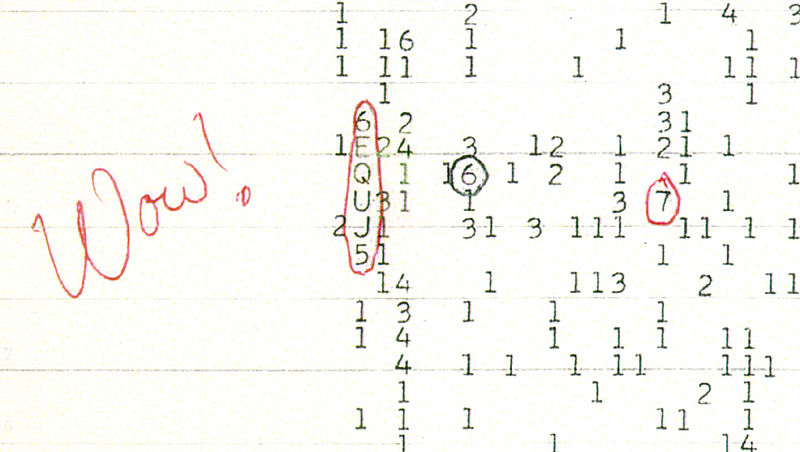
\includegraphics[width=\textwidth]{wow-signal.jpg}
\end{center}

\textbf{What is 6EQUJ5?}

The intensity is measured between 0 and 35.
Instead of just using numbers we changed 0 into a space and each number after 9 with the corresponding letter of the English alphabet.
For example A=10, B=11, Q=26 and U=30
\end{tcolorbox}